


\section{Pirate Game}
\label{sec:pirate}

\begin{emph}
On selecting the problem...
\end{emph}


\subsection{Problem Description}
\label{subsec:description}

The original Pirate Game is a multi-player version of the Ultimatum game that was first published as a mathematical problem in the Scientific American as a mathematical problem posed by Omohundro\cite{Stewart1999}. The main objective of the Pirate Game was to present a fully explainable problem with a non-obvious solution. The problem can be formulated as it follows:

\begin{quotation}
Suppose there are 5 rational pirates: A; B; C; D; E. The pirates have a  loot of 100 indivisible gold coins to divide among themselves.


As the pirates have a strict hierarchy, in which pirate A is the captain and E has the lowest rank, the highest ranking pirate alive will propose a division. Then each pirate will cast a vote on whether or not to accept the proposal. 

If a majority or a tie is reached the goods will be allocated according to the proposal. Otherwise the proposer will be thrown overboard and the next pirate in the hierarchy assumes the place of the captain. 

We consider that each pirate privileges her survival, and then will want to maximize the number of coins received. When the result is indifferent the pirates prefer to throw another pirate overboard and thus climbing in the hierarchy. 
\end{quotation}

\subsection{Analysis}
\label{subsec:analysis_PG}

We can arrive at an equilibrium in this problem by using backward induction. At the end of the problem, supposing there are two pirates left, the equilibrium is very straight forward. This sub-game is represented in Table \ref{tab:classico2jogadores}, and its Nash Equilibrium is $(C,D)$.



As the highest ranking pirate can pass the proposal in spite of the other decision, her self-interest dictates that she will get the 100 gold coins. Knowing this, pirate E knows that any bribe other higher ranking pirate offers her will leave her better than if the game arrives to the last proposal. 


\begin{table}
\begin{center}
\begin{centering}
\begin{tabular}{ccc}
\hline 
  & Player 2: C & Player 2: D\tabularnewline
\hline 
Player 1: C & (100, 0) & (100, 0)\tabularnewline
Player 1: D & (100, 0) & (-200, 100.5)\tabularnewline
\hline 
\end{tabular}

\par\end{centering}
\caption{Representation of the $2$ player sub-game in normal form.}
\end{center}
\label{tab:classico2jogadores}
\end{table}


\begin{table}
\begin{center}
\begin{tabular}{cc}
  \num\putindeepbox[7pt]{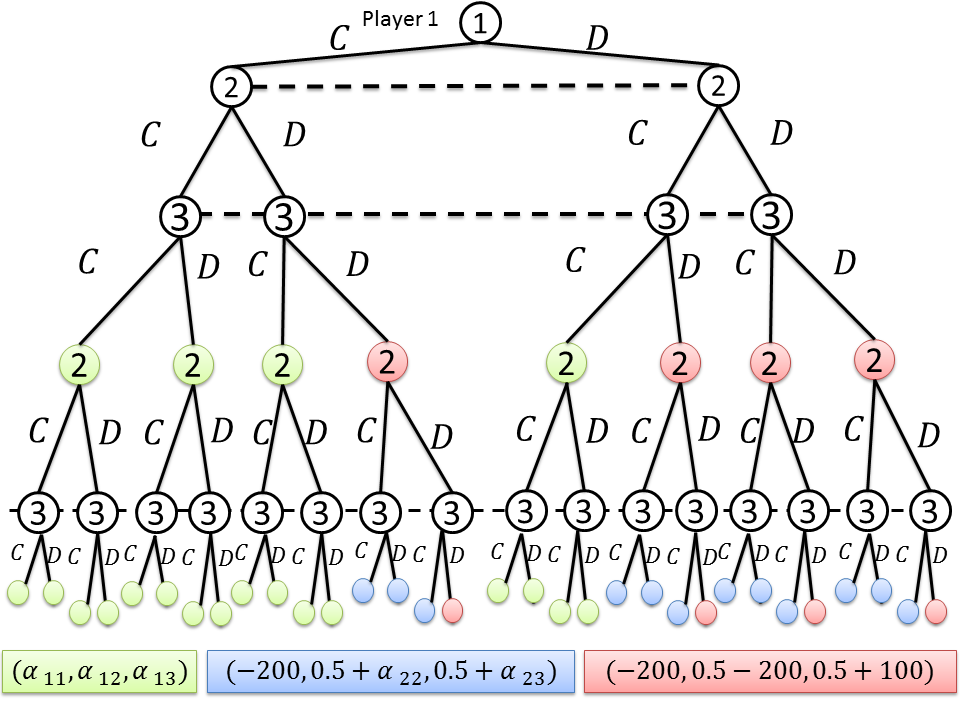
\includegraphics[scale=0.20]{Pirates1/Slide1.PNG}}
    & \num\putindeepbox[7pt]{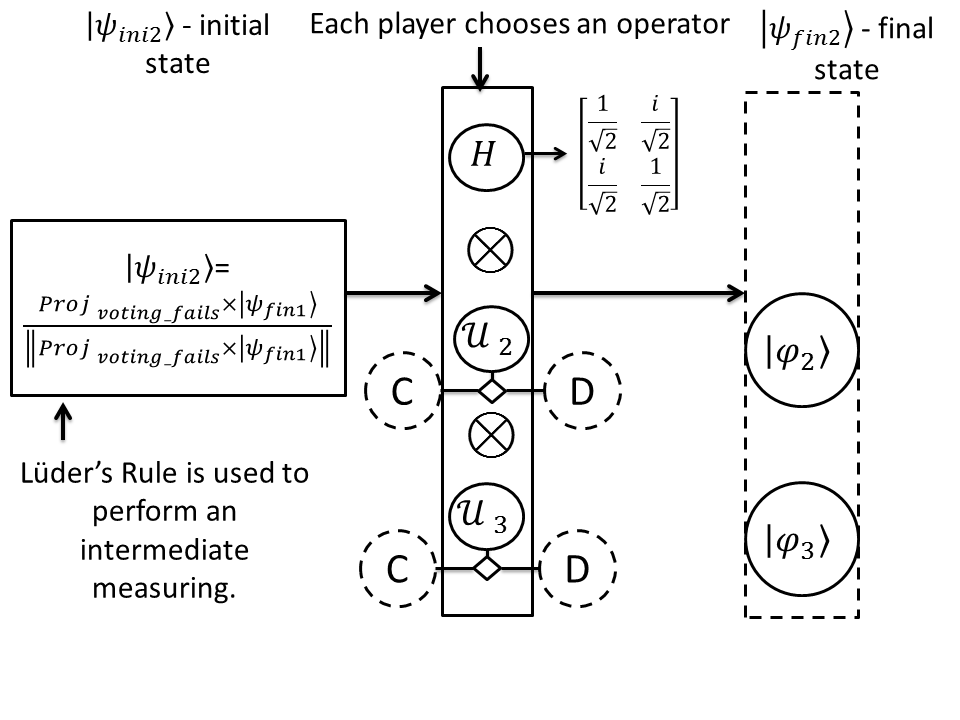
\includegraphics[scale=0.20]{Pirates1/Slide2.PNG}} \\
  \num\putindeepbox[7pt]{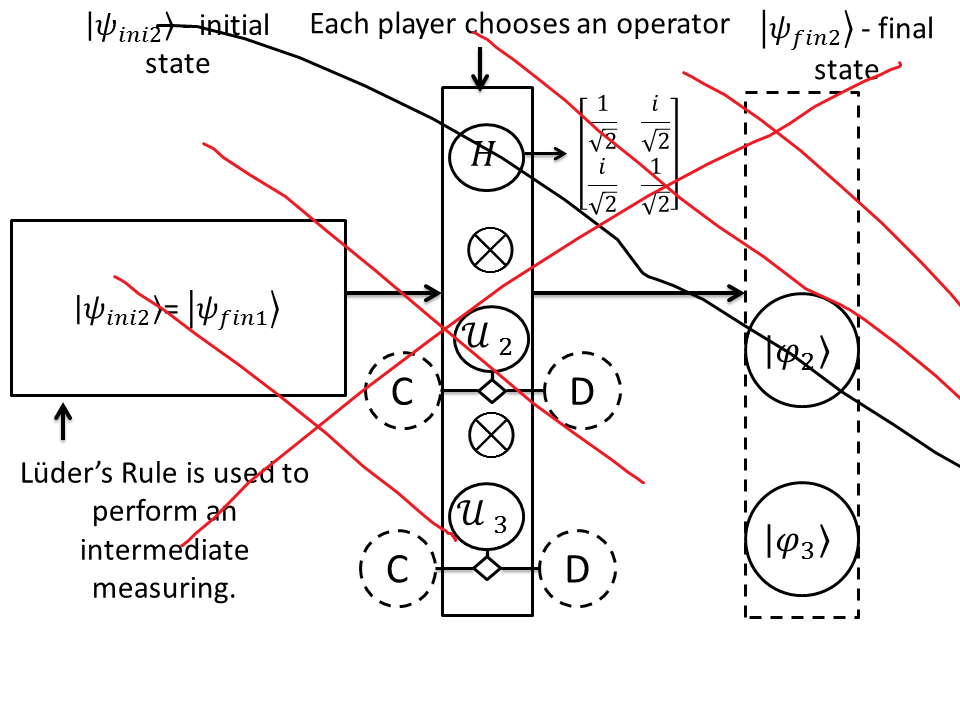
\includegraphics[scale=0.20]{Pirates1/Slide3.PNG}}
    & \num\putindeepbox[7pt]{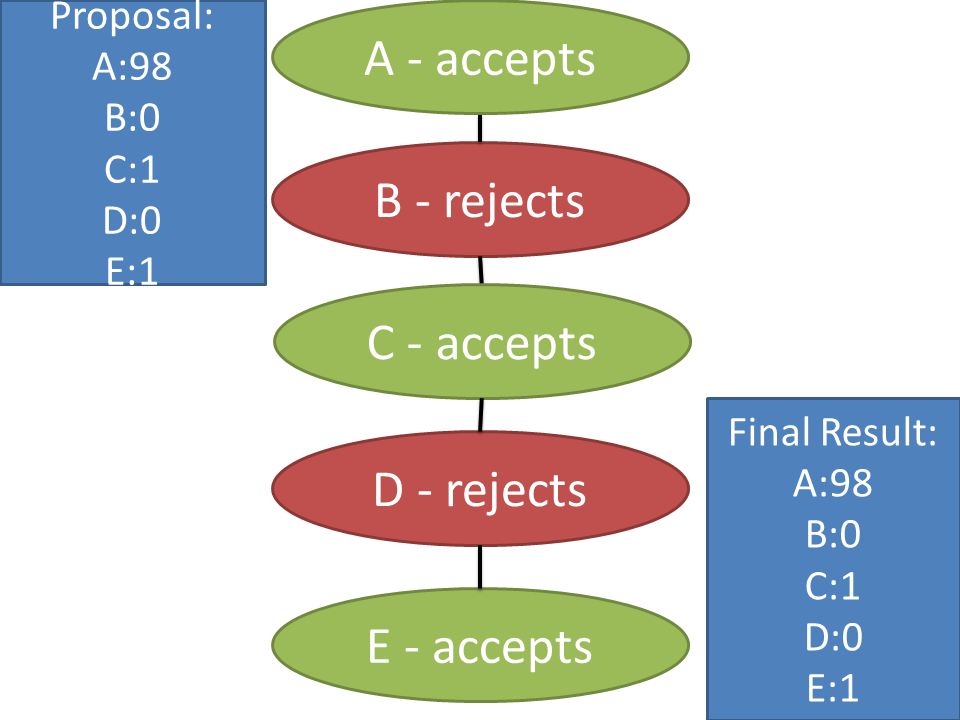
\includegraphics[scale=0.20]{Pirates1/Slide4.PNG}} \\
\end{tabular}
\caption{The equilibrium for the Pirate Game can be found through backward induction. From a), where there's only two pirates left, to d), that corresponds to the initial problem we define the best response.}
\label{tab:piratas_m}
\end{center}
 \end{table}

When applying this reasoning to the three pirate move, as pirate C knows she needs one more vote to pass her proposal and avoiding death, she will offer the minimum amount of coins that will make pirate E better off than if it comes to the last stage with two pirates. This means that pirate C will offer 1 gold coin to pirate E, and keep the remaining 99 coins. 

With 4 pirates, B would rather bribe pirate D with 1 gold coin, because E would rather like climb on the hierarchy and getting the same payoff. Finally, with 5 pirates the captain (A), will keep 98 gold coins and rely on pirate C and E to vote in favour of the proposal, by giving 1 gold coin each.

We can generalize this problem for $N$ pirates. If we assign a number to each pirate, where the captain is number 1 and the lower the number the higher the rank. If the number of coins is superior to the number of pirates, the equilibrium will have the captain (highest ranking pirate), giving a gold coin to each odd pirate, in case the number of players alive is odd, while keeping the rest to herself. When we have a even number of players the captain will assign a gold piece to each pirate with a even number, and the the remaining coins to herself. 

If the number of pirates is greater than two times the amount of coins $N>2C$, a new sittuation arises. If we have 100 coins and 201 pirates, the captain will not get any coin. By the same reasoning with 202 pirates the captain will still be able to survive by bribing the majority of the pirates and keeping no coins for herself. With 203 pirates the first captain will die. However with 204 pirates, the first captain will be able to survive even though he won't be able to bribe the majority, because her second in command knows that when she makes a proposal, she'll be thrown off board. In the game with 205 pirates, however the captain is not able to secure the vote from the second in command on the 204 pirate game, because the second captain is safe and she is able to make a have her proposal accepted and have the third pirate safe. 

We can generalize this problem for $N>2C$ as \cite{Stewart1999}, as the games with a number of pirates equal to $2C$ plus a power of two will have an equilibrium in the first round, in the others every captain until a subgame with a number of pirates equal to $2C$ plus a power of two will be thrown off board.

